\originalchapter{语言模型训练与推理}\label{ch:lm}
\originalsection{从序列概率到训练目标}
语言模型要给任意文本序列概率. 将文本切为 token 后, 序列为 $x_1,\ldots,x_T$. 由条件概率反复展开,
\[
p_\theta(x_{1:T})=\prod_{t=1}^T p_\theta(x_t\mid x_{<t}),\qquad
\mathcal L(\theta)=-\frac1T\sum_{t=1}^T\log p_\theta(x_t\mid x_{<t}).
\]
$x_{<t}$ 表示之前的全部 token. 零概率前缀的条件分布需要额外约定; softmax 模型对有限词表每步给正概率, 不会出现此问题. 文档边界可用开始与结束符表达, 是否跨文档拼接训练要明确.

Token 可以是字节、字符、词或子词. 词表大可缩短序列, 但增加输出矩阵和稀有 token 的学习负担; 词表小可处理陌生字符串, 但序列更长. BPE 迭代合并常见相邻单位, 其分词器应只从训练数据学习. Token 概率不是词概率, 不同分词下困惑度不可直接比较.

\begin{definition}
若平均负对数似然为 $\mathcal L$, 困惑度为 $\operatorname{PPL}=e^{\mathcal L}$. 它是按几何平均正确 token 概率定义的有效分支量, 不是模型每步实际考虑的候选个数.
\end{definition}
训练时称为 teacher forcing: 每个位置输入真实前缀, 同一批可并行预测所有下一 token. 推理时之前 token 来自模型自身, 必须逐步生成, 一个错误还可能改变后续条件分布. 这解释了低逐 token 损失与完整回答正确之间为什么存在距离.

\originalsection{CPU 小模型的完整训练闭环}
这里的完整指数据生成、前向、反向、优化与评价代码齐全. 它是数学实验用的简化因果注意力语言模型, 并非完整标准 Transformer.
首版使用原创有限语法, 文档均为八个词:
\begin{center}\texttt{<bos> cat sees red dog says meow <eos>}\end{center}
主语取 cat 或 dog, 颜色取 red 或 blue, 干扰动物取 cat 或 dog, 叫声由主语确定. 共八种组合, 词表含十个 token. 固定六种训练, 另两种留出, 不把同一文档的窗口分到两边. 模型宽度为 16, 单头因果注意力, 残差前馈层宽度为 32, 激活为 $\tanh$, 可学习 token 和位置向量. 省略归一化, 总参数量为 2,538.

输入是每篇前七个 token, 目标是后七个 token. 在输入位置 \texttt{says} 的输出处评价叫声, 因而正确预测需要获取之前主语而不是只看当前词. 基线统计训练集中 \texttt{says} 后的叫声频率, 无法按主语区分. 主语可独立于干扰动物, 这提供了测试检索依赖的机会.

模型使用全批次 Adam, 1,400 步, 步长 0.01, $\beta_1=0.9,\beta_2=0.999,\epsilon=10^{-8}$. 每步先将整体梯度范数裁剪到至多 1, 再更新一二阶量. 固定种子并不保证不同硬件和数值库位级相同, 所以环境版本和误差容限都记录在结果目录. 图 \ref{fig:lm} 来自已运行结果.
本次实际执行的训练平均交叉熵为 $0.2560$, 两个留出组合的平均交叉熵为 $1.5066$. 叫声位置准确率为 $100\%$, 只看最后一个词的基线为 $50\%$. 各参数组抽样梯度检查的最大误差为 $5.38\times10^{-11}$, 因果前缀检查的最大 logit 差为 $0.0$. 这些数值仅对应当前代码、种子与划分.
\par

\begin{figure}[ht]
\centering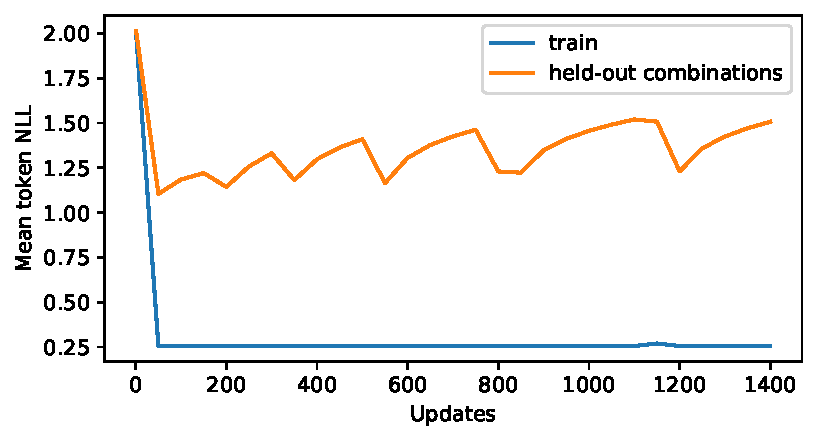
\includegraphics[width=.66\textwidth]{generated/language_model.pdf}
\caption{固定训练组合与两种留出组合的平均 token 交叉熵. 测试损失上升提示过拟合, 局部叫声任务正确并不等于整句泛化成功.}\label{fig:lm}
\end{figure}

即使训练充分, 全部 token 的平均损失也不应降到零. 训练集中相同开始前缀之后出现多个主语, 相同主语后也有多种颜色与干扰动物. 给定前缀 $c$, 令训练后继频率为 $\hat p(y\mid c)$, 对任何概率模型的该前缀平均损失均为 $H(\hat p, q)=H(\hat p)+\KL(\hat p\Vert q)$. 所以按前缀出现次数加权的经验条件熵构成不可越过的下界. 本划分的计算下界约为 0.2560, 训练损失已接近它, 而测试损失明显更高. 不能因训练损失没有为零就判断优化失败.

这份模型有三个可复核检查: 参数组梯度与有限差分相符; 改未来 token 不影响之前 logits; 只替换干扰动物后检查叫声预测. 本划分中将两个测试样本的干扰动物翻转后, 恰好得到训练中出现的组合, 因而此替换只检验该局部依赖, 不能当成进一步的新组合泛化证据. 注意力图可以帮助提出机制假说, 但只在两个样本上的成功和一个随机种子, 远远不足以证明稳定的组合泛化. 没有额外数据、模型规模或自然语言能力被包含在这些结果里.

\originalsection{推理分布与 KV 缓存}
贪心解码选每步最大概率 token, 速度简单, 但局部最优并不保证整条序列概率最大. 温度采样使用 $q_i(\tau)=\exp(z_i/\tau)/\sum_j\exp(z_j/\tau)$, $\tau>0$. 温度小使分布更集中, 大则更平坦; 它改变采样分布, 不修改模型权重. Top-$k$ 只保留最高的 $k$ 个 token 后归一化; top-$p$ 保留累计概率达到指定阈值的最小前缀. 两者都可能排除正确但低概率的候选, 不能直接解释为“提高智力”.

自回归推理分为 prefill 与 decode. Prefill 处理已有提示, decode 逐 token 生成. 每一层把过去的键和值缓存下来, 新 token 只生成自己的 $q,k,v$ 并读取缓存. 在因果掩码下旧位置不会因未来新增 token 改变, 所以缓存有效. 对常规多头模型, 忽略元数据, KV 元素数量约为 $2LTd$, 其中 $L$ 为层数, $d$ 为各头维度总和, $T$ 为缓存长度. 分组查询注意力共享部分键值头, 可以降低这一量. 缓存不是完整历史的无损语义压缩; 上下文截断或缓存淘汰会改变模型可读取的信息.

\originalsection{后训练}
预训练学习语料分布. 监督微调在输入--输出示例上继续最大似然, 让模型更适合指令形式. 人类反馈路线常先训练偏好奖励模型, 再优化生成策略; DPO 则在特定偏好与正则化建模假设下直接优化成对响应目标, 不需要显式运行奖励模型的强化学习回路\cite{instruct,dpo}. 二者都不能保证每个回答真实或安全.

若有参考策略 $\pi_{\rm ref}$ 与奖励 $r$, 常见序列目标为 $\E_{y\sim\pi}[r(x,y)]-\beta\KL(\pi\Vert\pi_{\rm ref})$. 在固定 $x$、有限候选集合且参考概率全正时, 将约束 $\sum_y\pi(y)=1$ 加入拉格朗日式, 对 $\pi(y)$ 求导可得 $\pi^*(y)\propto\pi_{\rm ref}(y)e^{r(x,y)/\beta}$. 正则化使策略不能免费地偏离参考分布. 真实训练需近似采样、估计和参数化, 不等同于直接求出此闭式分布.


\originalsection{低秩微调与偏好目标}
如果全模型微调成本过高, 可以冻结原矩阵 $W_0\in\R^{m\times d}$, 仅学习低秩更新 $\Delta W=BA$, 其中 $B\in\R^{m\times r},A\in\R^{r\times d}$, $r\ll\min(m,d)$. 新映射为 $(W_0+BA)x$. 可训练参数从 $md$ 变成 $r(m+d)$, 不计偏置. LoRA 使用这一参数化并配合缩放\cite{lora}. 它限制更新的矩阵秩, 不保证所有目标都能由低秩变化表达, 也不意味着训练激活内存全部消失. 若下游梯度为 $u$, 则 $\nabla_B\ell=u(Ax)^\top$, $\nabla_A\ell=B^\top u\,x^\top$.

前面的有限候选 KL 最优策略可不用只依赖驻点. 令
$q(y)=\pi_{\rm ref}(y)e^{r(y)/\beta}/Z$, $Z=\sum_y\pi_{\rm ref}(y)e^{r(y)/\beta}$. 直接展开相对熵得到
\[
\E_\pi[r]-\beta\KL(\pi\Vert\pi_{\rm ref})
=\beta\log Z-\beta\KL(\pi\Vert q).
\]
由相对熵非负且等号条件, 唯一最大值在 $\pi=q$. 参考概率全正、奖励有限与 $\beta>0$ 保证 $q$ 是合法全正分布. 这也说明正则化参数不是任意装饰: 当 $\beta$ 小, 策略更集中于高奖励; 当 $\beta$ 很大, 策略接近参考.

DPO 再假定成对偏好服从 Bradley--Terry 模型: 候选 $y_w$ 胜过 $y_l$ 的概率为 $\sigma(r(y_w)-r(y_l))$. 由最优分布关系, 奖励可写成
$r(y)=\beta\log[\pi^*(y)/\pi_{\rm ref}(y)]+\beta\log Z$. 两候选相减时 $\log Z$ 抵消. 用参数策略代替未知最优策略, 对胜者--败者对作最大似然, 得
\[
\begin{aligned}
\mathcal L_{\rm DPO}(\theta)
&=-\E_{(y_w,y_l)}\log\sigma(s_\theta),\\
s_\theta
&=\beta\left(\log\frac{\pi_\theta(y_w)}{\pi_{\rm ref}(y_w)}
 -\log\frac{\pi_\theta(y_l)}{\pi_{\rm ref}(y_l)}\right).
\end{aligned}
\]
这是偏好建模与 KL 正则化假设下的推导, 不是任何人类偏好数据都满足这些假设的证明. 人类评判可能噪声很大、不传递或依赖上下文; 参数策略也可能无法表示最优分布.

本项目 \texttt{preference} 用八个动作、已知奖励与非均匀参考分布, 按 Bradley--Terry 概率生成带噪偏好, 再训练八个 logit. 令 $\pi=\softmax(z)$, 对数策略比的差消去了 softmax 归一化, 所以
$s=\beta[(z_w-\log\pi_{{\rm ref},w})-(z_l-\log\pi_{{\rm ref},l})]$.
单对损失对 $z_w,z_l$ 的导数分别是 $-\beta\sigma(-s)$ 与 $\beta\sigma(-s)$, 其他坐标为零. 程序使用这个梯度, 并把真实奖励与 KL 分开报告, 再与解析最优目标比较. 有限带噪数据导致差距正常存在; 偏好损失更低不必然在所有新任务上效用更高.

\originalsection{练习与解答}
\begin{exercise}
输入三个 token $(a,b,c)$, 以每个位置预测下一 token, 第三目标为结束符. 写出目标序列和因果可见范围.
\end{exercise}
\begin{solution}
目标为 $(b,c,\texttt{<eos>})$. 第一位置只能看 $a$, 第二位置看 $a,b$, 第三位置看 $a,b,c$. 若第一位置看到了 $b$, 就把自己的目标作为输入泄漏了.
\end{solution}
\begin{exercise}
对 logits $(0,\log3)$, 比较温度 1 和温度 $1/2$ 的分布. 为什么这不能证明第二种设置更可靠?
\end{exercise}
\begin{solution}
温度 1 给 $(1/4,3/4)$, 温度 $1/2$ 给 $(1/10,9/10)$. 它只加强了原模型排序; 若原本高分候选是错的, 降温也会更自信地错. 可靠性要在独立任务上检验.
\end{solution}
\label{ch:end:08}
